\documentclass[a4paper,10pt]{article}

\usepackage{tabularx} % extra features for tabular environment
\usepackage{amsmath}  % improve math presentation
\usepackage{graphicx} % takes care of graphic including machinery
\usepackage[margin=1in,letterpaper]{geometry} % decreases margins
\usepackage{cite} % takes care of citations
\usepackage[final]{hyperref} % adds hyper links inside the generated pdf file
\usepackage{ctex}
\usepackage{titlesec}
%\usepackage{CJKutf8, CJK}
\usepackage{makecell}                 % 三线表-竖线
\usepackage{booktabs}                 % 三线表-短细横线
% \usepackage{natbib}
\usepackage{graphicx}				  % 表格单元格逆时针
\usepackage{multirow}				  % 合并单元格
\usepackage{array}
\usepackage{amssymb}				  % 勾
\usepackage{amsmath}
\usepackage{longtable}                % 导入 longtable 宏包,表格自动换行
\usepackage{caption}
\usepackage{subcaption}               % 设置子图
\usepackage{color}					  % 文本颜色包
\usepackage{xcolor}
\usepackage{bbm}					  % 输入指示函数
\usepackage{tablefootnote}			  % 表格注释
\usepackage{pythonhighlight}
\usepackage{fancyhdr}
\usepackage{lastpage}
\pagestyle{fancy}
\fancyhf{}
\fancyhead{}
\fancyfoot{}
\fancyhead[R]{\small Page \thepage\ of \pageref*{LastPage}}
\fancyhead[L]{\small Report}

\usepackage{listings}                 % 导入代码块
\usepackage{xcolor}
\lstset{
	numbers=left, 
	tabsize=1,
	columns=flexible, 
	numberstyle=  \small, 
	keywordstyle= \color{ blue!70},
	commentstyle= \color{red!50!green!50!blue!50}, 
	frame=shadowbox, % 阴影效果
	rulesepcolor= \color{ red!20!green!20!blue!20} ,
	escapeinside=``, % 英文分号中可写入中文
	xleftmargin=2em,
	xrightmargin=2em, 
	aboveskip=1em,
} 

\hypersetup{
	colorlinks=true,       % false: boxed links; true: colored links
	linkcolor=blue,        % color of internal links
	citecolor=blue,        % color of links to bibliography
	filecolor=magenta,     % color of file links
	urlcolor=blue         
}
%++++++++++++++++++++++++++++++++++++++++
\titleformat{\section}{\Large\bfseries\songti}{\thesection}{1em}{}
\titleformat{\subsection}{\large\bfseries\songti}{\thesubsection}{1em}{}
\titleformat{\subsubsection}{\normalsize\bfseries\songti}{\thesubsubsection}{1em}{}
\titleformat{\paragraph}{\small\bfseries\songti}{\paragraph}{1em}{}
\titleformat{\subparagraph}{\footnotesize\bfseries\songti}{\subparagraph}{1em}{}

\begin{document}
	
	
	\title{\songti \zihao{4}Unity VR 项目开发进度}
%	\author{\textrm{Ku Jui}}
	\date{\textrm{January 2024}}
	\maketitle
	
	\renewcommand{\figurename}{Figure} % 可以重新定义abstract,因为ctex会覆盖thebibliography
	% 	\begin{abstract}
		%		In this experiment we studied a very important physical effect by measuring the
		%		dependence of a quantity $V$ of the quantity $X$ for two different sample
		%		temperatures.  Our experimental measurements confirmed the quadratic dependence
		%		$V = kX^2$ predicted by Someone's first law. The value of the mystery parameter
		%		$k = 15.4\pm 0.5$~s was extracted from the fit. This value is
		%		not consistent with the theoretically predicted $k_{theory}=17.34$~s. We attribute %this
		%		discrepancy to low efficiency of our $V$-detector.
		%	\end{abstract}
	\renewcommand{\contentsname}{Contents}
	\renewcommand{\tablename}{Table}
	\tableofcontents  % 自动生成目录
		
	\section{开发进展}

		\subsection{PC 端软件界面}	
		
		VertiVR-CDP Tester(PC端)软件界面如 Fig. \ref{fig:vertivr-cdp-tester-ui} 所示,单击蓝牙开关启动蓝牙功能(需要 Windows 端启动蓝牙开关),随后单击 Find Device 按钮搜索周围蓝牙设备,如 Fig. \ref{fig:vertivr-cdp-tester-finddevice}所示。随后我们选择可以选择支持蓝牙串口协议的设备,单击 Connect 按钮进行连接。
		
		我们在另外一台 PC 设备上构建了支持蓝牙串口协议的环境,我们通过串口调试软件验证了 PC 端通过蓝牙串口协议发送指令的可行性。如 Fig. \ref{fig:serial-port-assistant} 所示,我们通过蓝牙串口不断的向 VertiVR-CDP Tester 发送数据 43 01 02,分别代表电量67,大版本号 1,小版本号 2,VertiVR-CDP Tester 界面能够显示从蓝牙串口接收到的数据包并进行解析,如 Fig. \ref{fig:vertivr-cdp-tester-connect} 所示。此外,我们分别依次单击 Darkness, Senthrough, Freeze Pitch, Set Pitch 按钮,在串口调试助手上,我们依次接收到5个数据包。
		
		我们对蓝牙缓冲区的定义如 Table. \ref{tab: bluetooth-buffer-definition} 所示。
		\begin{table}[!htbp]
			\centering
			\tiny
			\begin{tabular}{>{\centering\arraybackslash}m{2.6cm}|c|c}
				\hline
					
				\textbf{Byte} & \textbf{Instruction} & \textbf{Definition} \\
					
				\hline
					
				0 & 软件次版本号     & \multirowcell{2}{\centering value 表示传递的值}\\ 
				1 & 软件主版本号     & \\ 
					
				\hline
					
				2 & Seethrough      & \multirowcell{3}{\centering 0x80表示激活,0x00 表示不激活}\\
				3 & Darkness        & \\
				4 & Freeze Pitch    & \\
					
				\hline
					
				5 & Pitch 值(-10-10)& \multirowcell{2}{\centering 0x80表示未激活,value 表示传递的值}\\
				6 & Scene(0-3)      & \\
					
				\hline
					
				7 & \multirowcell{2}{\centering -} & \multirowcell{2}{\centering 保留} \\
				8 &                & \\
				\hline		
			\end{tabular}
			\caption{\label{tab: bluetooth-buffer-definition}
				蓝牙缓冲区的定义
			}
		\end{table}

		\begin{figure}[htbp] 
			\centering 
			\begin{subfigure}{0.23\textwidth}
				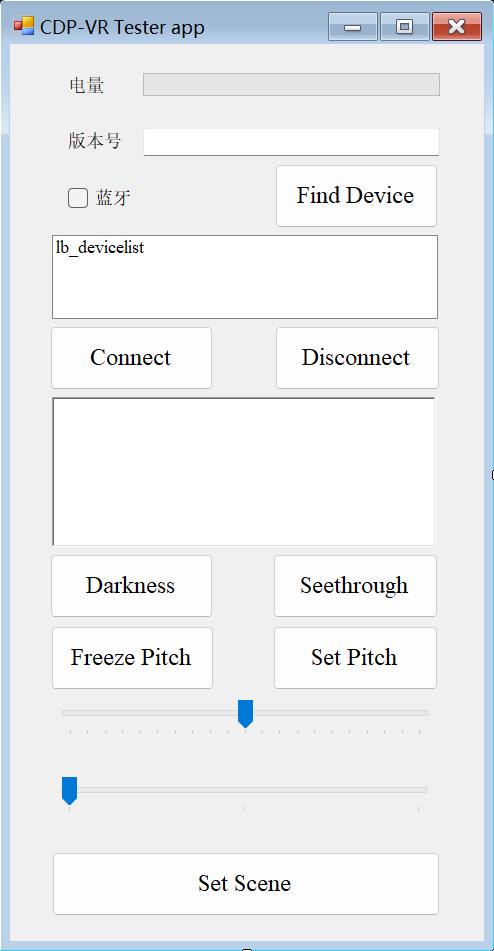
\includegraphics[width=\linewidth]{picture/VertiVR-CDP Tester UI}
				\captionsetup{font=scriptsize}
				\caption{PC端软件界面}
				\label{fig:vertivr-cdp-tester-ui}
			\end{subfigure}
			\begin{subfigure}{0.23\textwidth}
				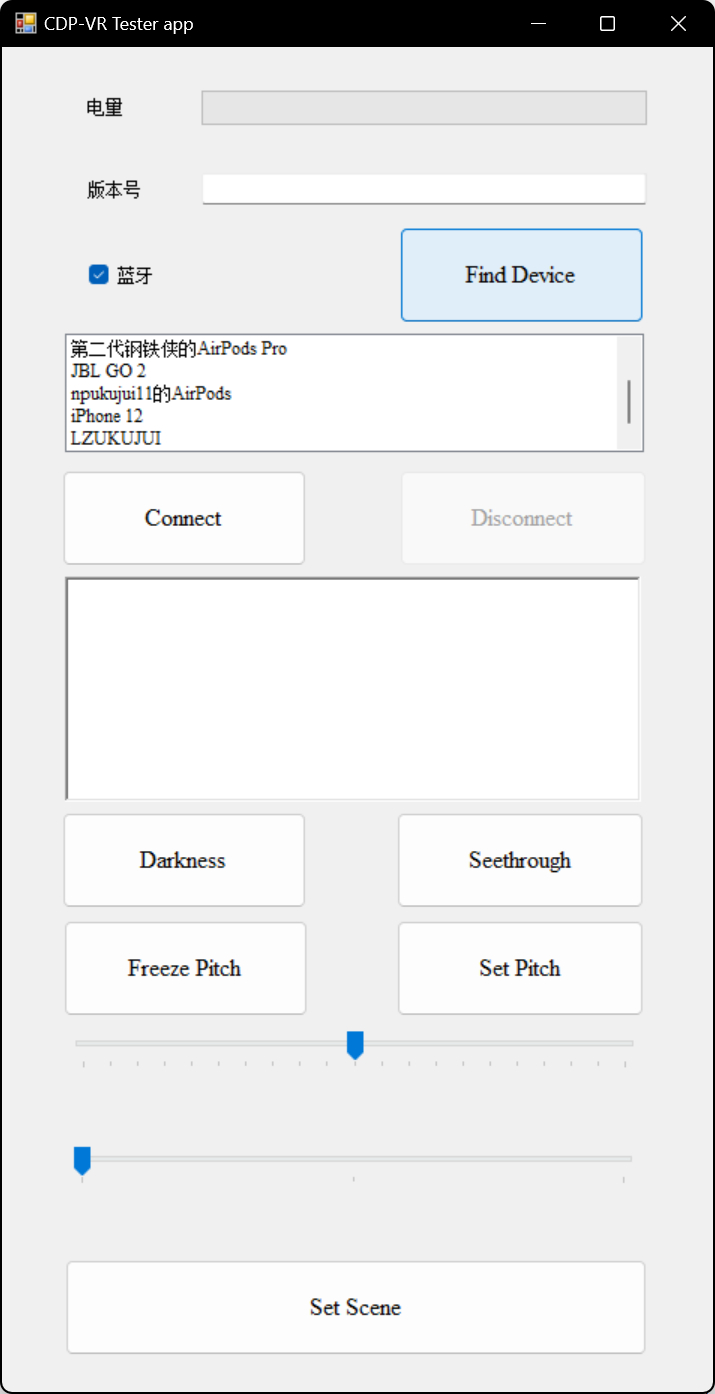
\includegraphics[width=0.98\linewidth]{picture/VertiVR-CDP Tester FindDevice}
				\captionsetup{font=scriptsize}
				\caption{软件运行后的界面}
				\label{fig:vertivr-cdp-tester-finddevice}
			\end{subfigure}
			\begin{subfigure}{0.23\textwidth}
				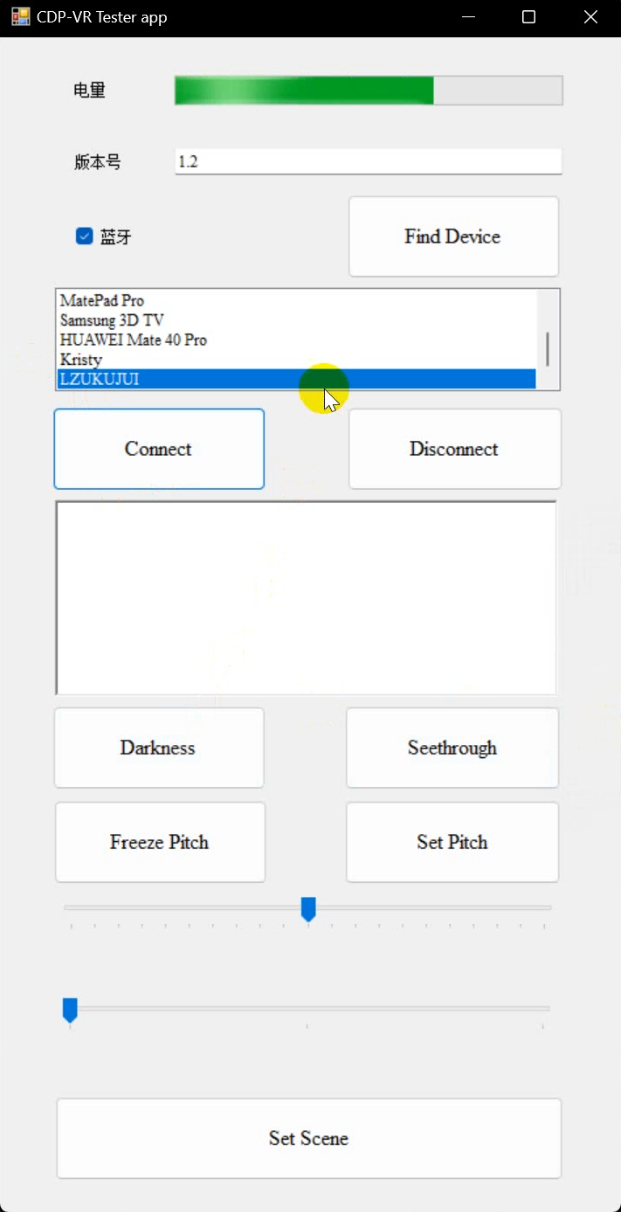
\includegraphics[width=0.98\linewidth]{picture/VertiVR-CDP Tester Connect}
				\captionsetup{font=scriptsize}
				\caption{建立连接后的界面}
				\label{fig:vertivr-cdp-tester-connect}
			\end{subfigure}
%			\captionsetup{font=scriptsize}
			\caption{
				\label{fig: PC Main menu}	
				主界面示意图				
			}
		\end{figure}
	
		\begin{figure}[htbp]
			\centering
			\includegraphics[width=0.7\linewidth]{"picture/Serial Port Assistant"}
			\caption{串口调试助手}
			\label{fig:serial-port-assistant}
%			\captionsetup{font=scriptsize}
		\end{figure}
			
	
		\subsection{Pico 端软件界面}
		
		我们构建了软件的启动界面,通过点击 Setting 按钮来进入设置菜单界面。点击 Bluetooth 开关打开蓝牙功能。
		
		\begin{figure}[htbp] 
			\centering 
			\begin{subfigure}{0.49\textwidth}
				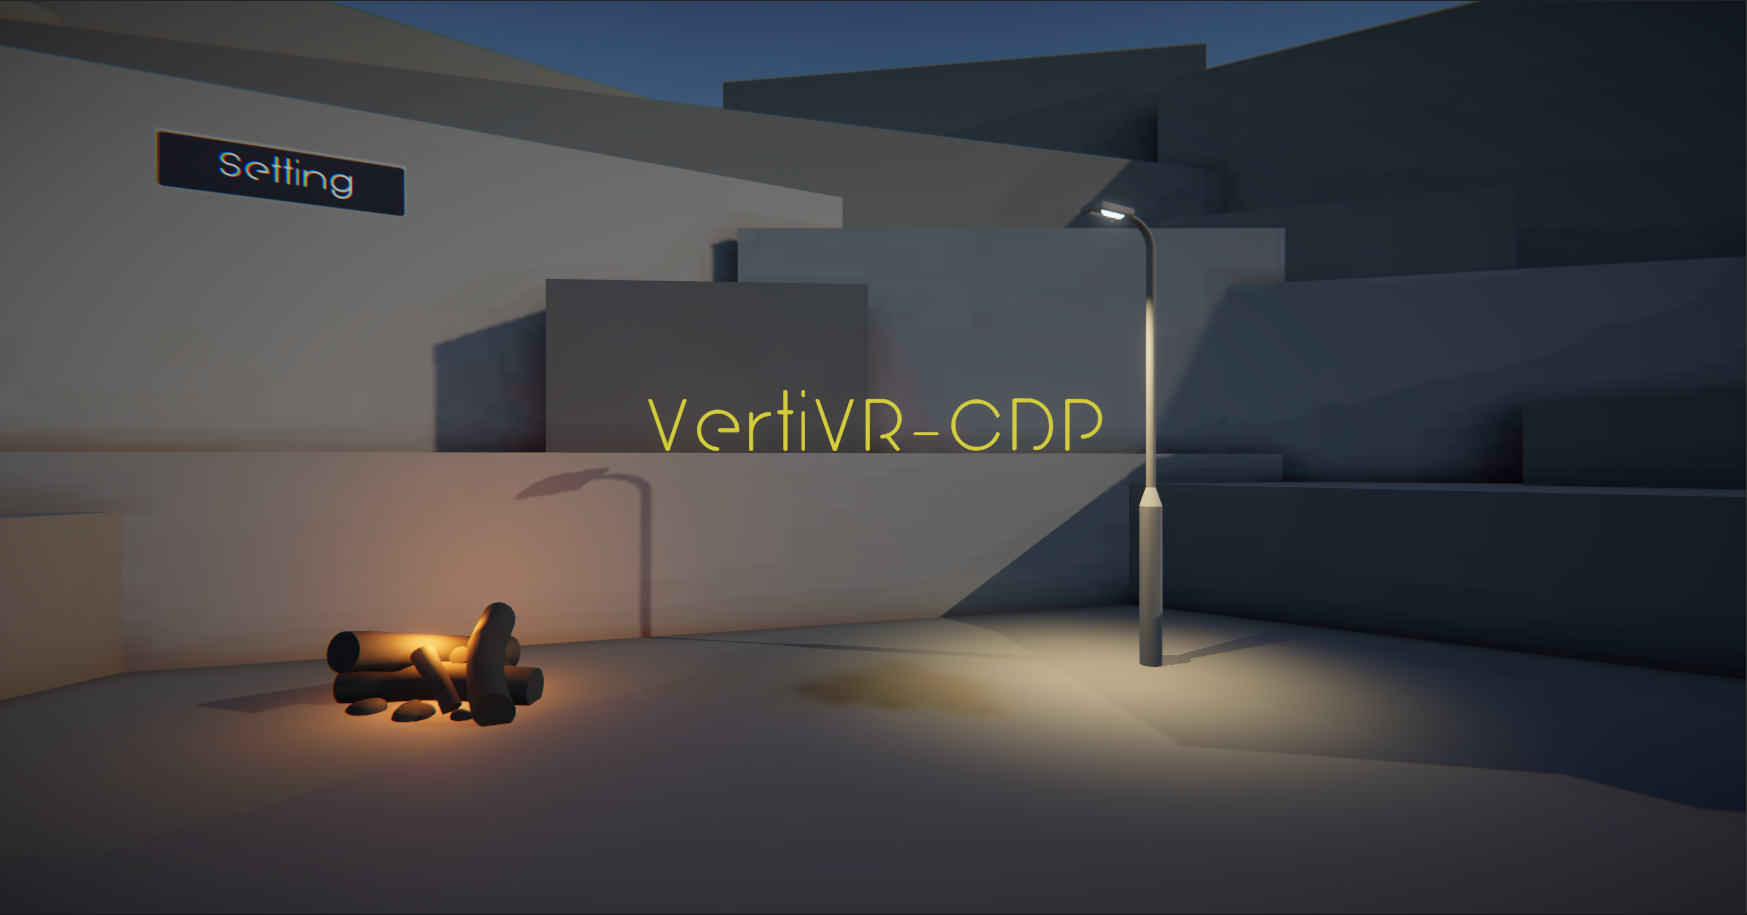
\includegraphics[width=\linewidth]{picture/Pico UI 1}
				\captionsetup{font=scriptsize}
				\caption{Pico 端软件界面1}
				\label{fig:pico-ui-1}
			\end{subfigure}
			\begin{subfigure}{0.49\textwidth}
				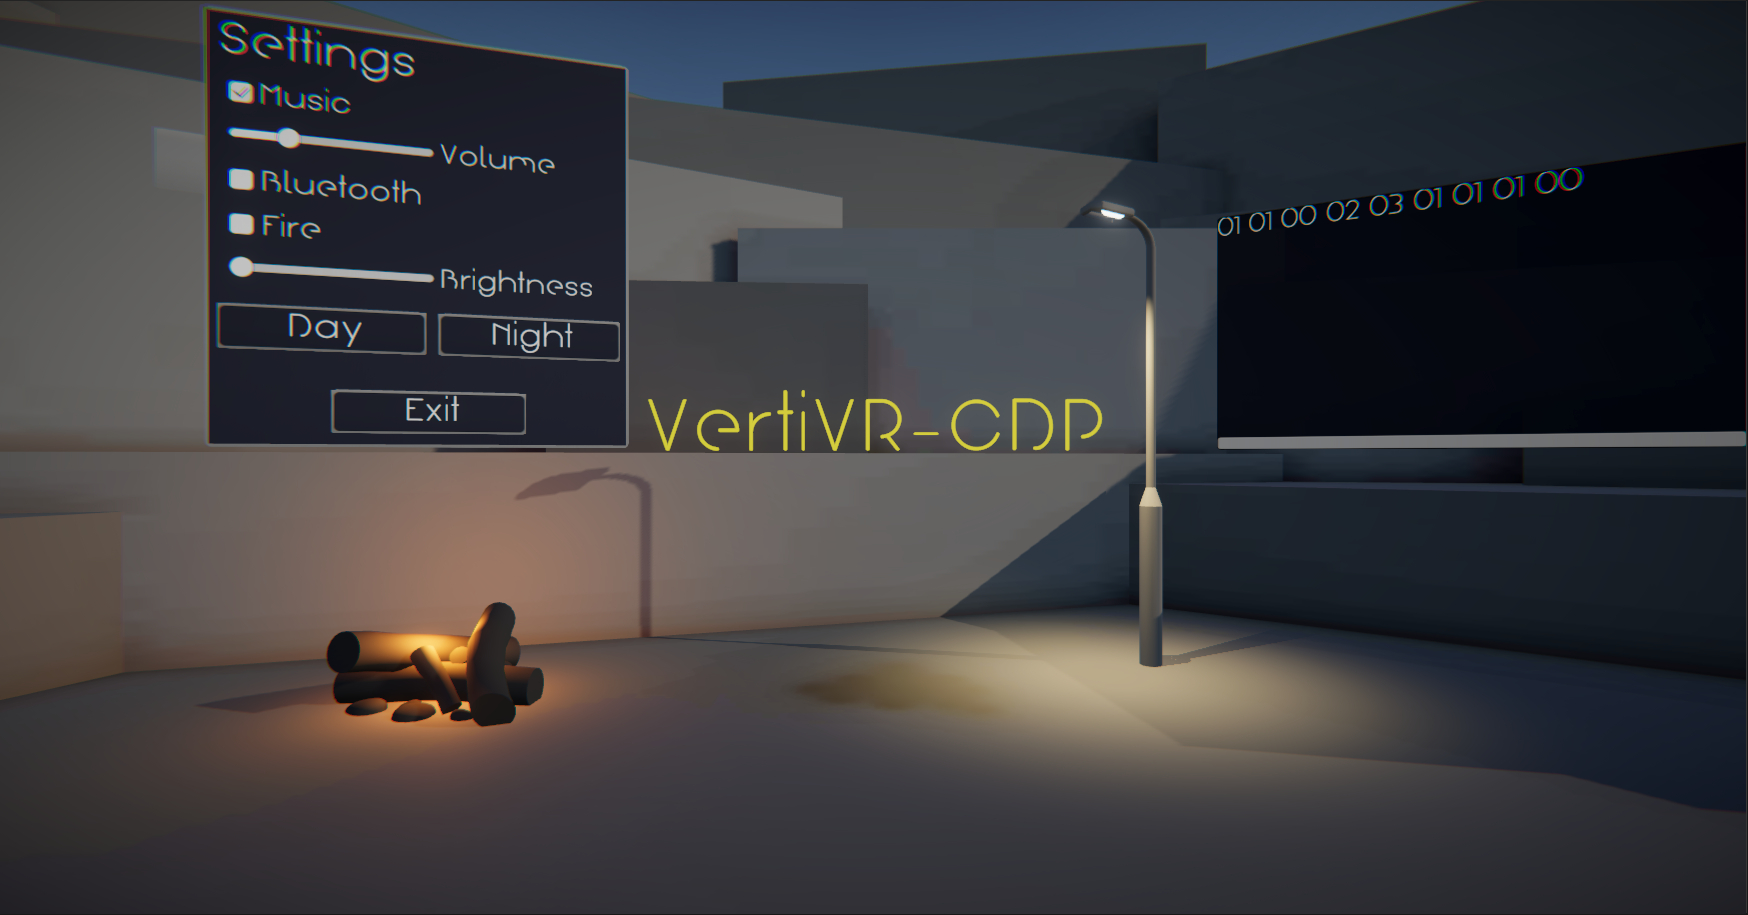
\includegraphics[width=\linewidth]{picture/Pico UI 2}
				\captionsetup{font=scriptsize}
				\caption{Pico 端软件界面2}
				\label{fig:pico-ui-2}
			\end{subfigure}
			%\captionsetup{font=scriptsize}
			\caption{
				\label{fig: Pico Main menu}	
				Pico 端主界面示意图				
			}
		\end{figure}
	
		\section{存在问题}
		
		目前 PC 端的功能已经基本实现,Pico 端的蓝牙功能并未实现。我们通过调研发现 Pico 端有\textbf{两种途径}可以实现蓝牙功能:
		
		\begin{itemize}
			\item[(1)] 一是使用 Unity Asset 提供的第三方蓝牙功能库,如 Fig. \ref{fig:unity-asset} 所示。
			\item[(2)] 二是基于 Android 平台的标准蓝牙 API 实现我们所需要的蓝牙串口功能,编译后生成 jar 包导入 Unity 使用。
		\end{itemize}

		\begin{figure}[htbp]
			\centering
			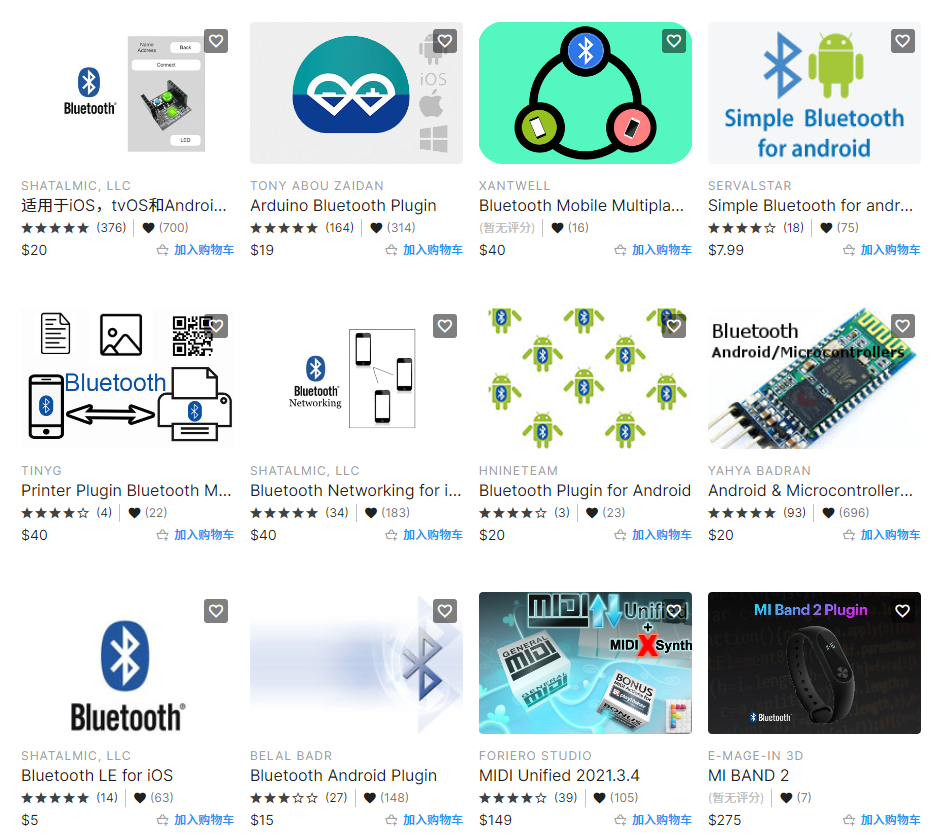
\includegraphics[width=0.5\linewidth]{picture/Unity Asset}
			\caption{Unity Asset 商店}
			\label{fig:unity-asset}
		\end{figure}
		
		但是考虑到第一种方法的花费的时间可能较少,所以一开始我们尝试采用第一种方法,使用第三方蓝牙库来完成蓝牙功能。		
		
		
%		\renewcommand{\refname}{References}
		
		
		%	\begin{thebibliography}{00}
			
			%		\bibitem{b1}\label{cite:b1}
			%		W. Wang, C. Wei, W. Yang and J. Liu, "GLADNet: Low-Light Enhancement Network with Global Awareness," 2018 13th IEEE International Conference on Automatic Face \& Gesture Recognition (FG 2018), Xi'an, China, 2018, pp. 751-755, DOI: 10.1109/FG.2018.00118.
			
			%		\bibitem{b2}\label{cite:b2}
			%		A.\ Mahajan, K.\ Somaraj and M. Sameer, "Adopting Artificial Intelligence Powered ConvNet To Detect Epileptic Seizures," 2020 IEEE-EMBS Conference on Biomedical Engineering and Sciences (IECBES), Langkawi Island, Malaysia, 2021, pp. 427-432, DOI: 10.1109/IECBES48179.2021.9398832.
			
			%		\bibitem{Cyr}
			%		N.\ Cyr, M.\ T$\hat{e}$tu, and M.\ Breton,
			% "All-optical microwave frequency standard: a proposal,"
			%		IEEE Trans.\ Instrum.\ Meas.\ \textbf{42}, 640 (1993).
			
			
			
			%	\end{thebibliography}
		
%		\bibliographystyle{unsrt}
%		\bibliography{reference}
		
		
	\end{document}
